\section{Postprocessing}
\begin{figure}[htb]
\noindent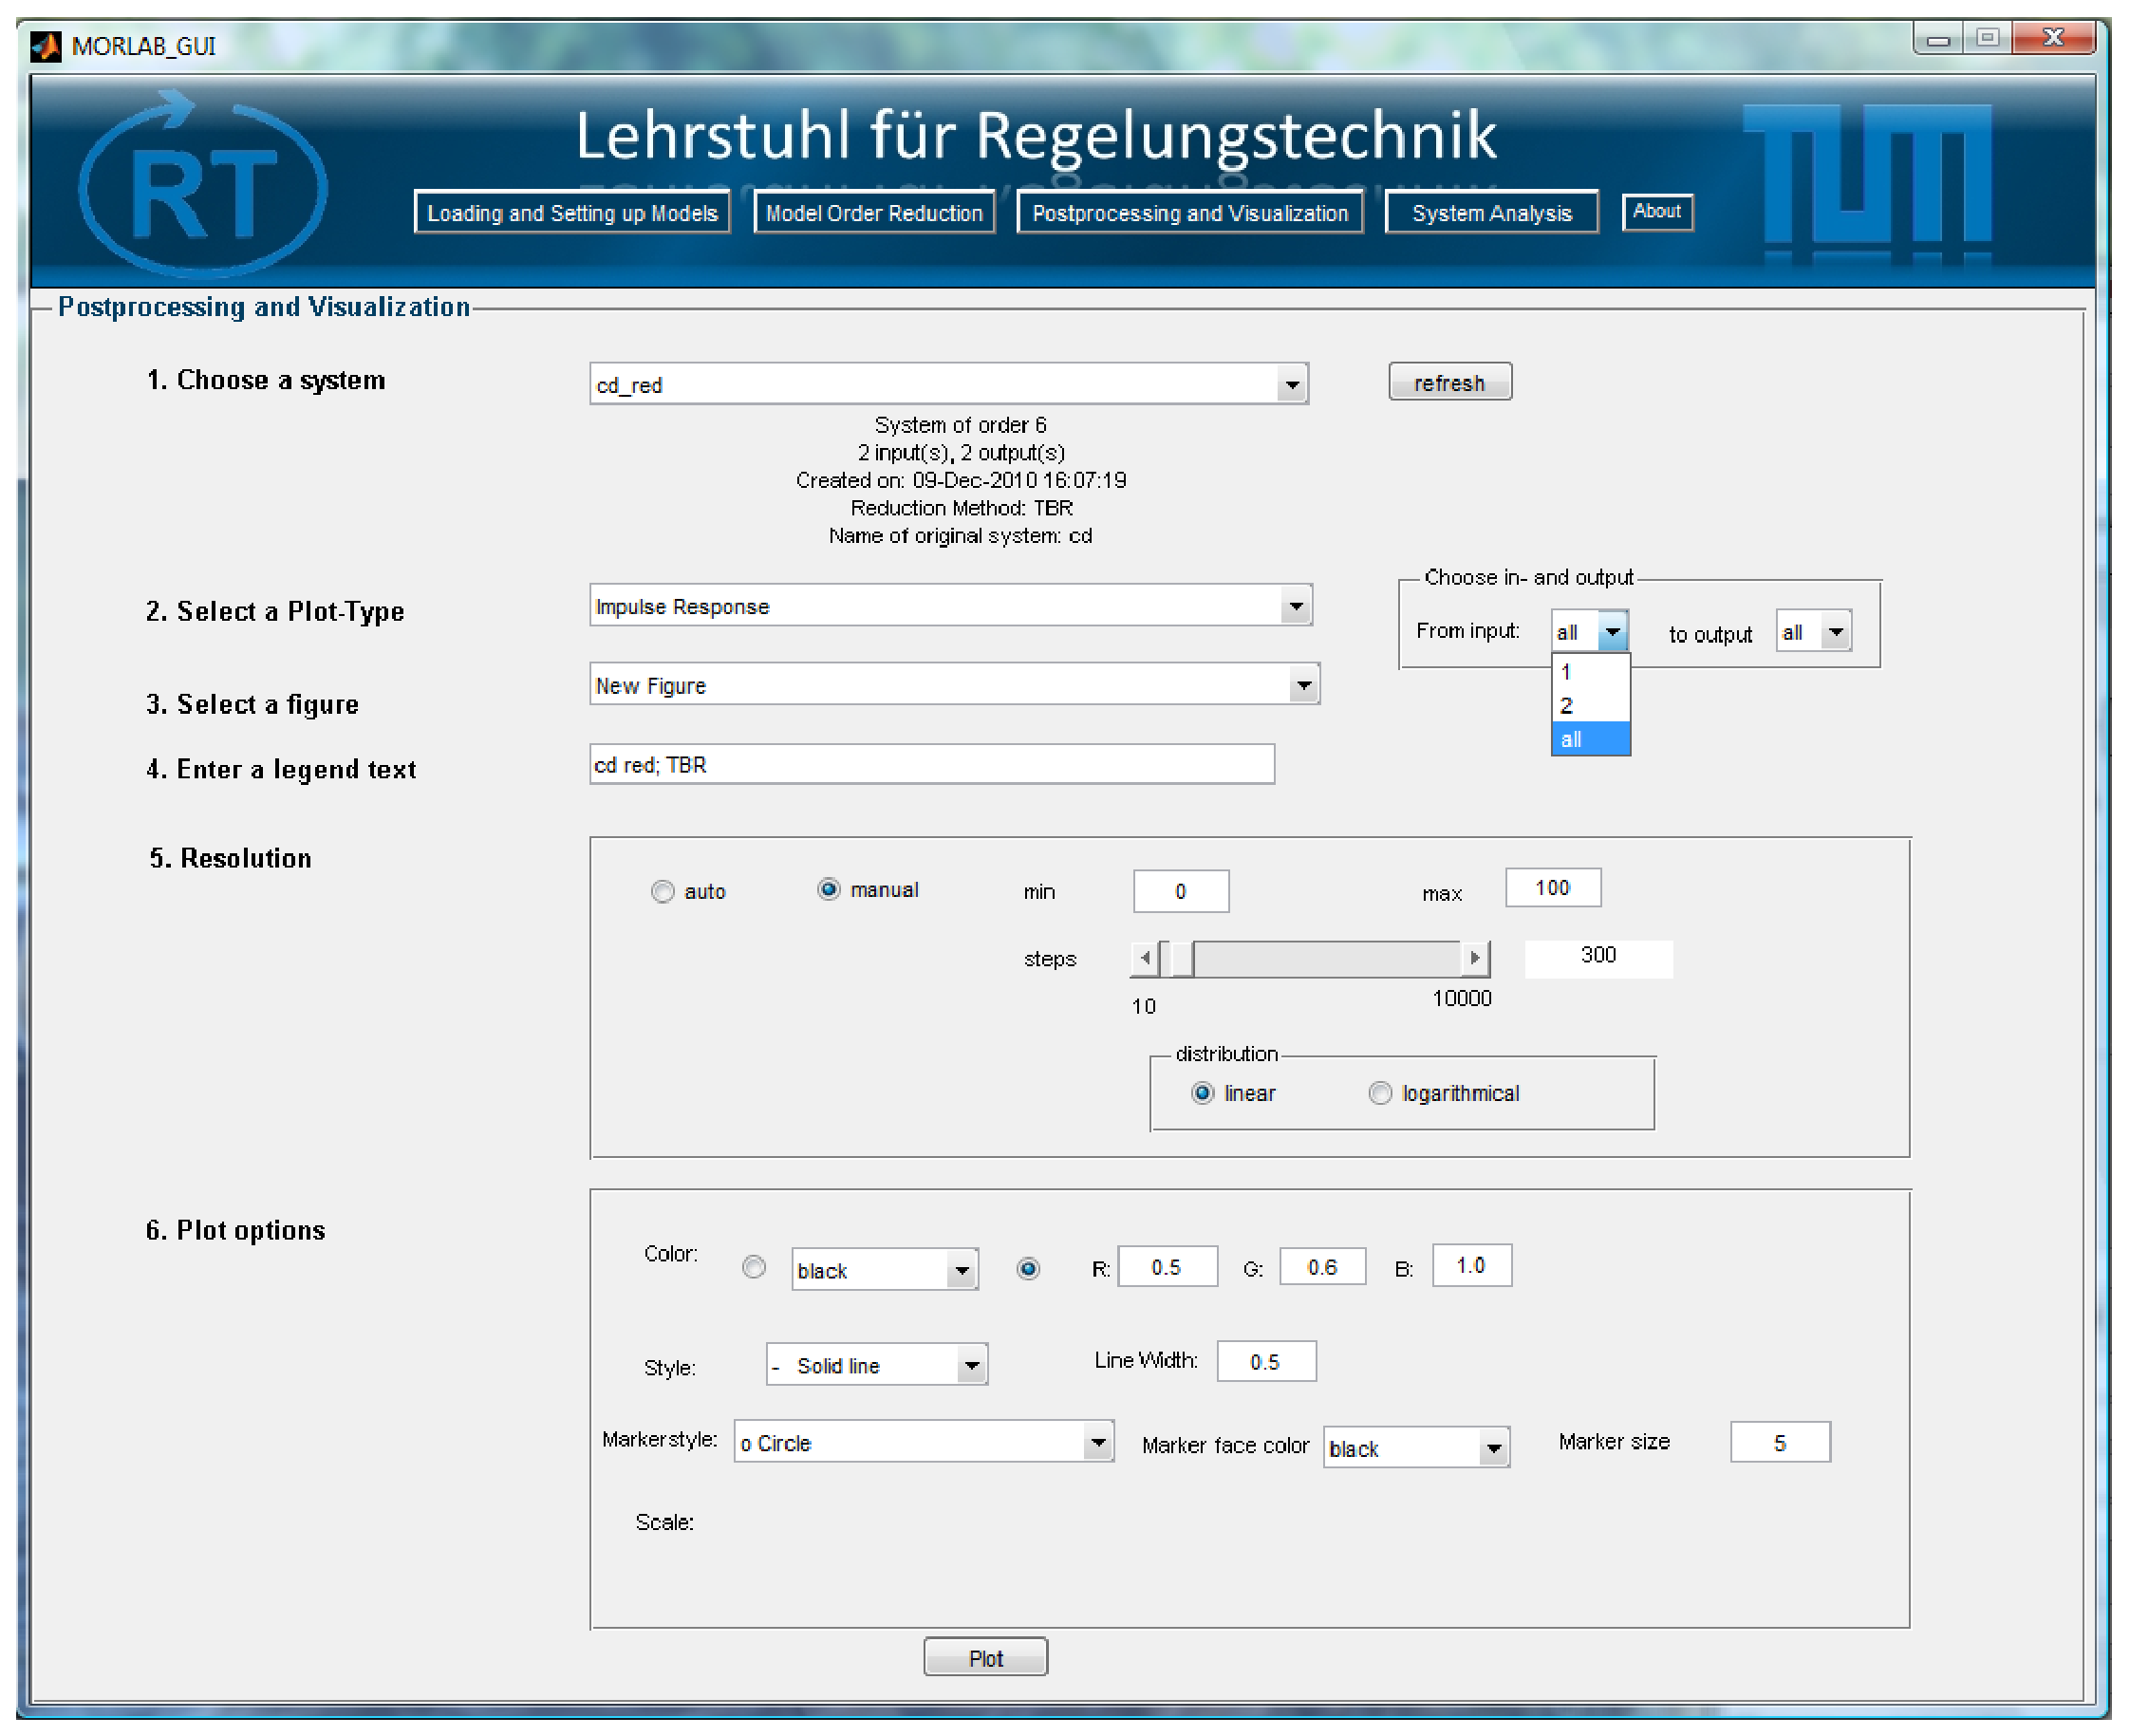
\includegraphics[width=\linewidth,keepaspectratio]{Abbildungen/tab_post}
\caption{Tab Postprocessing}
\end{figure}
Auf der "`Postprocessing and Visualization"' Seite k�nnen Impulsantwort, Sprungantwort, Bode Diagramm, Frequenzantwort und eine Polstellen/Nullstellen Karte erzeugt werden. (Abb.8)

\subsection{System ausw�hlen}
Zun�chst muss ein System ausgew�hlt werden. Dazu existiert, wie auch schon bei der Ordnugsreduktion eine Dropdown Liste. Im Textfeld unter der Liste erscheinen Informationen �ber das gew�hlte System.

\subsection{�bertragungsfunktion w�hlen}
Bei  MIMO-Systemen (multiple input multiple output) kann gew�hlt werden ob alle �bertragungsfuntionen ber�cksichtigt werden sollen, oder nur einzelne. F�r die Auswahl ist das Feld "`from in to out"' vorgesehen, welches nur sichtbar ist, wenn ein entsprechendes System gew�hlt wurde.

\subsection{Plot Typ w�hlen}
Unter "`Plot-Type"' kann ausgew�hlt werden, was erzeugt werden soll

\subsection{Figure ausw�hlen}
Zur Auswahl steht entweder eine neue Figure, oder eine in der sich bereits ein Graph des gleichen Typs befindet. So ist es zum Beispiel nicht m�glich ein Bodediagramm in eine Figure zu zeichnen, in der sich bereits eine Impulsantwort befindet.

\subsection{Legendentext festlegen}
Der Text, der im Textfeld "`legend text"' eingegeben wird, erscheint sp�ter in der Legende.

\subsection{Aufl�sung bestimmen}
Der Nutzer kann das Zeit- bzw. Frequenzintervall automatisch bestimmen lassen (Radiobutton "`auto"' im Resolution Feld) oder �ber "`manual"' Anfang und Ende des Zeit-/Frequenzbereichs eingeben, sowie die Zahl der zu Berechnenden Punkte. Die Verteilung der Punkte kann linear oder logarithmisch erfolgen. (Feld "`distribution"') 

\subsection{Layout des Graphen}
Im Feld "`Plot options"' kann das Layout des Graphen bestimmt werden. Die Farbe kann entweder �ber eine Dropdown-Liste, die die Standard Farben von Matlab enth�lt, oder durch Eingabe eine Farbvektors erfolgen.  Bei diesem werden die Intensit�ten von rot, gr�n und  blau in den Feldern "`R"',  "`G"' und "`B"' eingegeben. Die Werte m�ssen zwischen 0 und 1 liegen.